%----------------------------------------------------------------------------------------
%	PACKAGES AND OTHER DOCUMENT CONFIGURATIONS
%----------------------------------------------------------------------------------------

\documentclass[12pt]{article}
\usepackage[danish]{babel}
\usepackage{mathtools}
\usepackage[euler]{textgreek}
\usepackage[numbered,final]{mcode}
\usepackage[utf8x]{inputenc}
\usepackage{amsmath}
\usepackage{graphicx}
\usepackage[colorinlistoftodos]{todonotes}
\usepackage[toc,page]{appendix}
%\usepackage{float}
\usepackage{floatrow} % used for adding "Source" to pictures
\usepackage{hyperref} % used for hyperlinks
\usepackage[all]{hypcap}
\usepackage{bm} % used for bold inline matj
\usepackage{lipsum} % used for lorem lipsum
\usepackage[final]{pdfpages} % used for including PDF's
\usepackage{geometry}
\usepackage{listingsutf8}
\usepackage{listings}
\usepackage{blindtext}
\usepackage{enumitem}
\usepackage{color} %red, green, blue, yellow, cyan, magenta, black, white
\definecolor{mygreen}{RGB}{28,172,0} % color values Red, Green, Blue
\definecolor{mylilas}{RGB}{170,55,241}
\hypersetup{colorlinks=true, linkcolor=black}

% Page margins
\geometry{verbose,tmargin=1in,bmargin=1in,lmargin=1in,rmargin=1in,headsep=0.35in}

\begin{document}
	
	\begin{titlepage}
		
		
		
		\newcommand{\HRule}{\rule{\linewidth}{0.5mm}} % Defines a new command for the horizontal lines, change thickness here
		\setlength{\topmargin}{0in}
		\centering % Center everything on the page
		
		%----------------------------------------------------------------------------------------
		%	HEADING SECTIONS
		%----------------------------------------------------------------------------------------
		\textsc{\LARGE Aarhus universitet}\\[1.5cm] % Name of your university/college
		\textsc{\Large Adaptive Control and Automation}\\[0.5cm] % Major heading such as course name
		\textsc{\large 7. Semester}\\[0.5cm] % Minor heading such as course title
		
		%----------------------------------------------------------------------------------------
		%	TITLE SECTION
		%----------------------------------------------------------------------------------------
		
		\HRule \\[0.4cm]
		{ \huge \bfseries ACA projekt}\\ % Title of your document
		\HRule \\[1cm]
		
		%----------------------------------------------------------------------------------------
		%	AUTHOR SECTION
		%----------------------------------------------------------------------------------------
		
		\begin{minipage}{0.4\textwidth}
			\begin{flushleft} \large
				\emph{Gruppemedlemmer:}\\
				Søren Landgrebe \\
				Tim Hede Stenholt Jensen \\
			\end{flushleft}
		\end{minipage}
		~
		\begin{minipage}{0.4\textwidth}
			\begin{flushright} \large
				\emph{Studienr:} \\
				201508295\\
				201508449\
			\end{flushright}
		\end{minipage}\\[5cm]
		
		%----------------------------------------------------------------------------------------
		%	LOGO SECTION
		%----------------------------------------------------------------------------------------
		
		
\includegraphics[scale=0.5]{Img/logo.jpg}\\[1cm]
		
		%----------------------------------------------------------------------------------------
		%	DATE SECTION
		%----------------------------------------------------------------------------------------
		
		{\large \today}\\[0.5cm] % Date, change the \today to a set date if you want to be precise
		
		
		\vfill % Fill the rest of the page with whitespace
		
	\end{titlepage}
	
\newpage
\tableofcontents
\newpage
\listoffigures
\newpage

\hypersetup{linkcolor=blue}



%!TEX root = ../../Main.tex
\graphicspath{{Chapters/Indledning/}}
%-------------------------------------------------------------------------------

\section{Indledning}
Under optagelse til et live madprogram, sker det ofte at værten skal bruge en blender/foodprocesser. Dette betyder at værten ikke kan kommunikere med seerne mens blenderen/foodprocesseren kører. Denne problematik vil Noise Suppression System (NSS) kunne afhjælpe. Gennem en digital signal prossesering (DSP), vil vi dæmpe støjsignalet fra en køkkenmaskine dynamisk i realtid. Systemet består af to mikrofoner, et placeres tæt på støjen, et andet tæt på værten. De to mikrofoner fungere som input til vores system (Blackfin), hvor procceseringen og filtreringen foregår. Efter proceseringen bliver produktet afspillet på en højtaler, som erstatning for højtaleren fra et tv-apperat. Et overblik over systemet kan ses på figur \ref{fig:konceptbillede}

\begin{figure}[H]
	\centering
	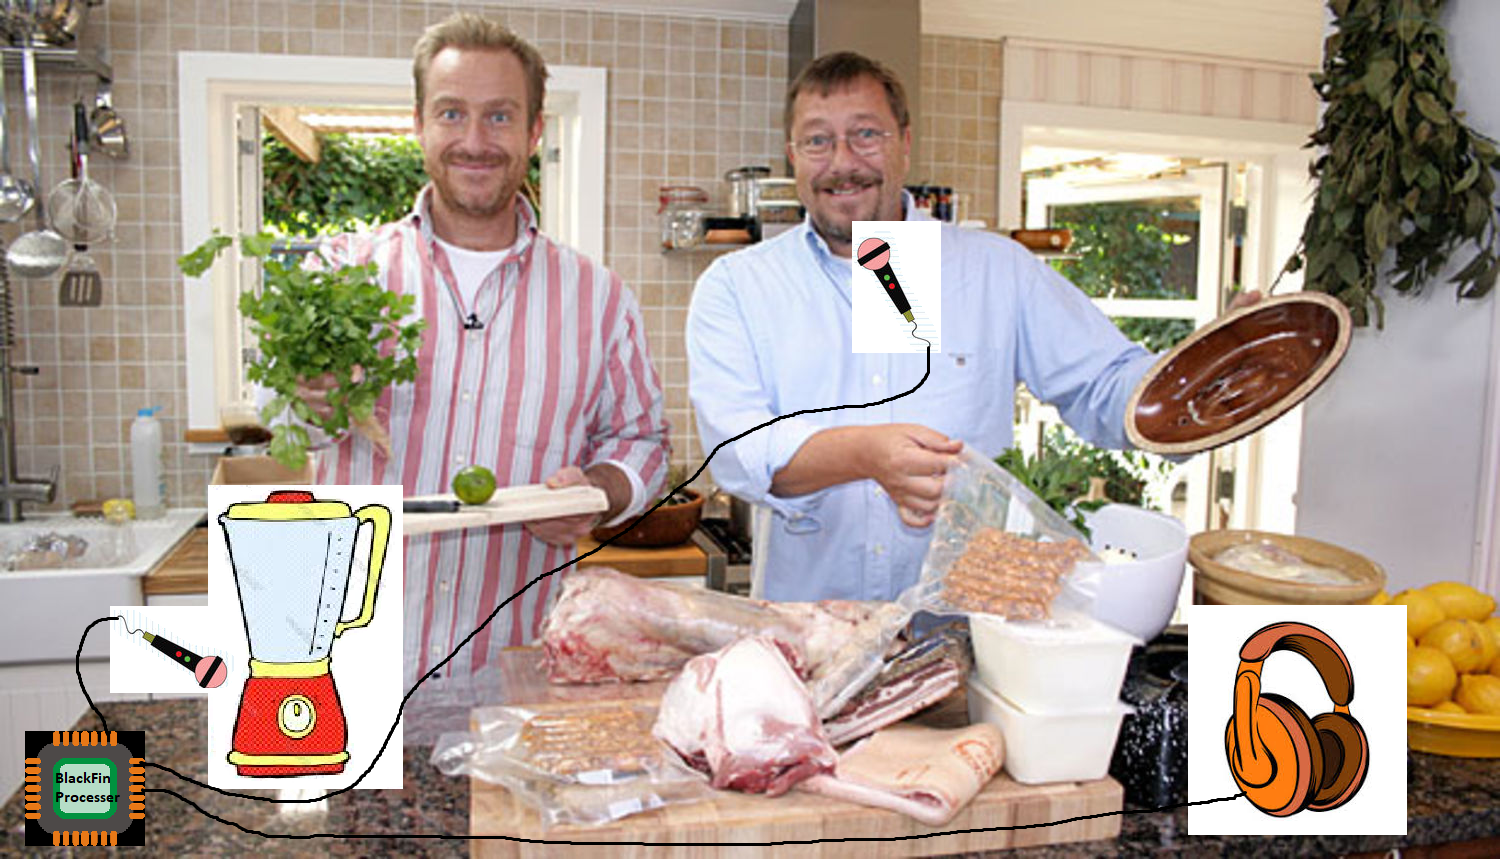
\includegraphics[width = 400pt]{Img/Konceptbillede}
	\caption{Konceptbillede for NSS}
	\label{fig:konceptbillede}
\end{figure}

Med udgangspunkt i brugerens behov vil der blive opstillet en række brugsscenarier, der beskriver brugerens interaktion med systemet. Disse scenarier vil sammen med en række veldefinerede krav og afgrænsninger, danne grundlaget for designet af alle dele af systemet.  \\ 

\newpage


	%!TEX root = ../../Main.tex
\graphicspath{{Chapters/Krav/}}
%-------------------------------------------------------------------------------


\section{Krav til dynamiken}
I dette afsnit beskrives kravene til hvilken funktionalitet systemet har. 


I samarbejde med vejleder er der opstillet en række krav.
\begin{itemize}
\item Systemet kan regulere en horisontal vinkel på op til ±30 grader tilbage til vandret i ”overdelen” ±1 grad
\item Overshoot max 5\%
\item Risetime 0.2 sekund 
\item Settlingtime 1 sekund 
\item Stadtionær fejl 10\%  

\end{itemize}



Herunder vil vi vise et blokdiagram, som viser en beksrivelse af systemets (fysiske) blokke, som beskriver opbygningen af systemet på Lego bilens styringsenhed. 


\begin{figure}[H]
	\centering
	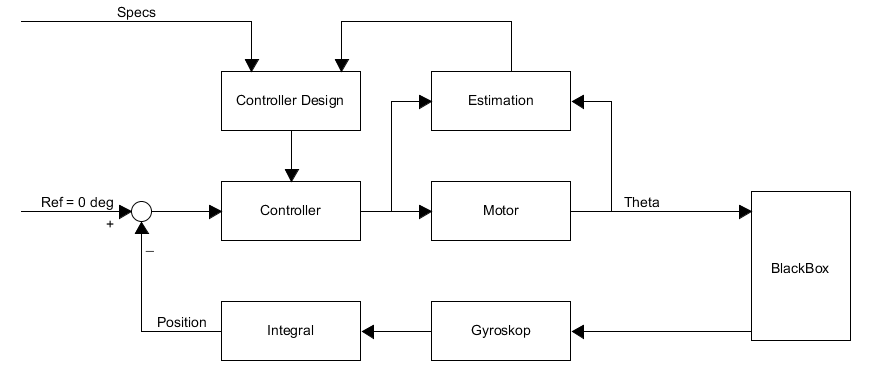
\includegraphics[width = 400 pt]{Img/blokdiagram.png}
	\caption{Blokdiagram}
	\label{fig:Blokdiagram}
\end{figure}

%!TEX root = ../../Main.tex
\graphicspath{{Chapters/Teori/}}
%-------------------------------------------------------------------------------


\section{Teori}
For at kunne estimere dette system, er det første som skal laves en overføringsfunktion, for den motor som bliver brugt til projeketet. Her stødte vi på det første problem med vores system, da det ikke var stabilt. Gruppen blev derfor nød til at indsætte fjedre, for at sikre at systemet var stabilt i en stationær position. Hertil blev der valgt at tilføje en elastik til hver side af bilen, for at opfylde ønsket om et stabilt stationær system. 
Herefter blev målingen lavet for at identificere, en overføringsfunktion for motoren. Da dette system, både skal kunne gå mod højre og venstre, blev der påført et firkantsignal. herunder ses, hvordan dynamikken i motorens tagometer blev genereret gennem firkantsignalet. (billedet mangler, da vi er ved at kigge på om vi hellere vil have det i grader)      
   

\begin{figure}[H]
	\centering
	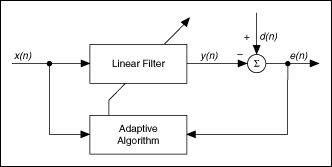
\includegraphics[width = 400pt]{Img/Figures}
	\caption{LMS adaptive filter}
	\label{fig:LMS_filter}
\end{figure}

På figur \ref{fig:LMS_filter} ses et overblik over det adative system, hvor x(n) er støjsignalet, y(n) er det filtrede støjsignal, med koefficienter som opdateres fra blokken "Adaptive Algoritm". d(n) er det ønskede signal inklusiv det støjende signal. e(n) er forskellen mellem d(n) og y(n) og derved støjen fratrukket fra det samlede signal af ønsket og støj.\cite{Teori}  \newline 


Det digitale filter bliver beregnet ud fra formlen:

\begin{equation}
  y(n) = \displaystyle\sum_{l=0}^{L-1} W(n)*x(n-1)
\end{equation}
Hvor W(n) er den værdi, som dynamisk opdateres. Dette sker ved at vi beregner den næste værdi ud fra formlen: 

\begin{equation}
  W(n+1) = W(n)-\mu *X(n)*e(n)
\end{equation}

Hvor W er den nye koefficient til filteret, X(n) er input signalet, og \textmu\ er en faktor, som bestemmer hastigheden af filteret, samt styrer infaldstiden. Hvis \textmu\ er lav bliver filteret langtsommere, mens settling time stiger jo højere vi kommer. Typisk må denne værdi ikke overstige 1. 
\newline
Dette giver os et endeligt udtryk som stemmer overens med figur \ref{fig:LMS_filter}, ift summeringspunktet: 
\begin{equation}
  e(n) = d(n)-y(n)
\end{equation} 

%!TEX root = ../../Main.tex
\graphicspath{{Chapters/Struktur/}}
%-------------------------------------------------------------------------------

\section{Struktur}

\subsection{BlackFin blokforklaring}

I dette projekt er der taget et valg udfra læringsmålene om at vi bruger Blackfin platformen til at udføre projektetes funktionalitet. Da en blackfin processor er bygget op af mange funktionalle blokke, vil der i det kommende afsnit laves et overblik over de interne forbindelser mellem hardware blokkene som bliver brugt i dette projekt. \cite{Struktur}

\begin{figure}[H]
	\centering
	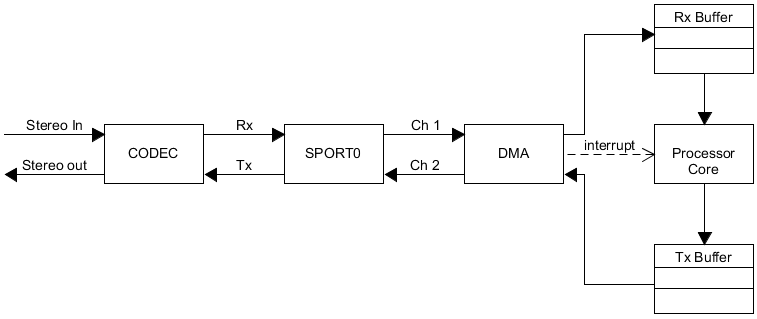
\includegraphics[width = 400pt]{Img/Struktur}
	\caption{Struktur NSS}
	\label{fig:Struktur}
\end{figure}

Igennem processen af vores funktionalitet, sendes lydsignalet gennem en codec1836, som har til opgave at sende inputtet gennem en ADC, hvorefter den sender det digitale signal videre til SPORT0, som står for at modtage og sende dataen. \\

DMA'en står for at sende dataen videre til Rx bufferen, når bufferen er fuld sender DMA'en interrupt til processeren om at procesere den modtagne data. \\
I den modsatte retning bliver det proceserede data flyttet til Tx bufferen, når Tx bufferen er fuld, sendes det til SPORT0 via DMA'en med Ch 2.  
Til sidst bliver dataen samplet gennem CODEC, som konverterer til et analogt signal vha. en DAC.
De forskellige blokke i strukturen fra figur \ref{fig:Struktur}, er implementeret i Init.C. 
  

\newpage

\subsection{Software arkitektur}
Til dette projekt har det været muligt at benytte et udleveret framework til Crosscore. Dette framework er lavet af Kim Bjerge, og er blevet modificeret af gruppen, til at virke med vores LMS filter. På \autoref{fig:Class diagram} kan man se hvilke klasser der er med i projektet og deres relationer til hinanden. 


\begin{figure}[H]
	\centering
	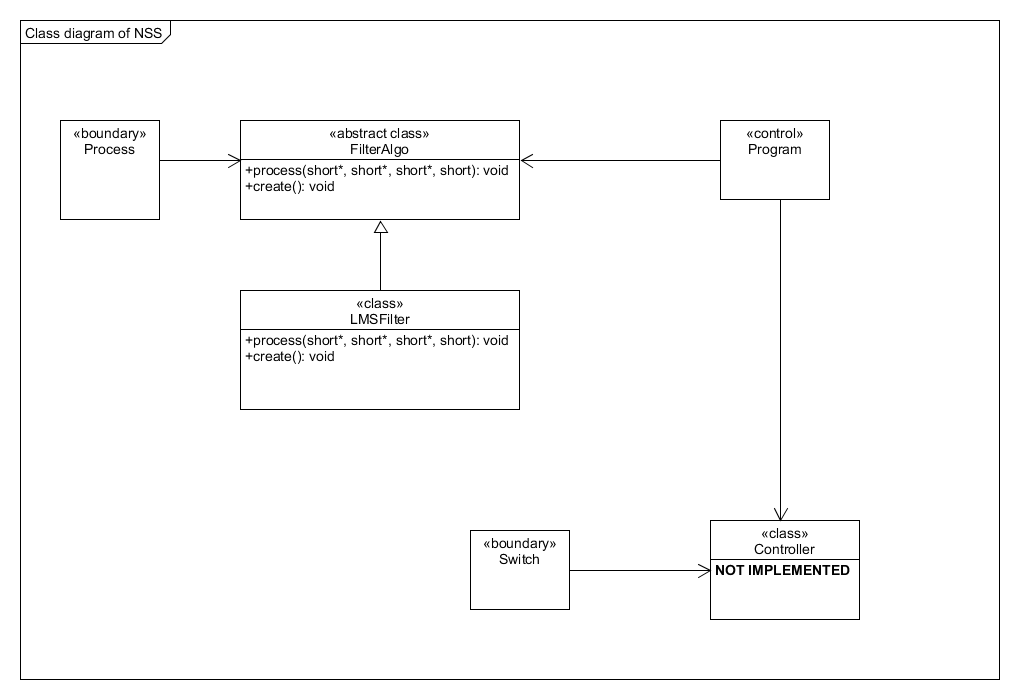
\includegraphics[width = 400pt]{Img/ClassDiagram.png}
	\caption{Klassediagram over NSS}
	\label{fig:Class diagram}
\end{figure}

Arkitekturen består af en abstrakt klasse FilterAlgo som har to virtuelle funktioner, process() og create(). Disse to nedarves af LMSFilter klassen og implementeres heri. Create() opretter filteret og nulstiller alle koefficienter, udover den første filter-koefficient, som bliver sat til 1. Grunden til dette er for at få det fulde støjsignal igennem første gang filteret kører. Dette vil blive uddybet mere i diskusion afsnittet. process() funktionen står for at filtrere uønsket støj fra tale signalet(d(n)). Koden er lavet så den følger vores matlab model så godt som overhovedet muligt. 

Vi har valgt ikke at implementere controller klassen, da vores 1. prioritet har været at få et fungerende LMS filter. Derfor står den som "NOT IMPLEMENTED". Istedet for at brugeren kan tænde for filteret med en switch, har vi valgt at lade filteret være aktiv så snart man starter programmet. 



\newpage


\begin{lstlisting}
for(short i = 0; i < len; i++)
{
	long fract yn = 0;

	for(short j = 0; j < NUM_WEIGTHS; j++)
	{
		if(i > j)
		{
			yn = yn + Filter.W[j]*x[i-j];
		}
	}
	y[i] = (fract)yn;
	e[i] = d[i] - yn;
		
	long fract tmp_W = 0;
		
	for(short k = 0; k < NUM_WEIGTHS; k++)
	{
		if(i > k)
		{
			Filter.W[k] = Filter.W[k]  + my*x[i-k]*e[i];
		}
	}
}
\end{lstlisting}

Koden ovenfor består af tre for-løkker. Den yderste løkke særger for at køre længden af signalet igennem. Løkken i linje 5, filtrere støjen så vi får vores støjsignal y(n). Dette støjsignal trækkes fra vores talesignal hvilket efterlader vores ønsket talesignal uden støj. Den sidste løkke på linje 17, opdaterer filter-koefficienterne så de hele tiden passer til støjen.

For at forsimple koden har vi valgt at splitte vores stereo kanal op i to, så det er muligt at få støjsignalet(x(n)) ind på højre kanal og tale signal(d(n)) ind på venstre kanal.


\begin{figure}[H]
	\centering
	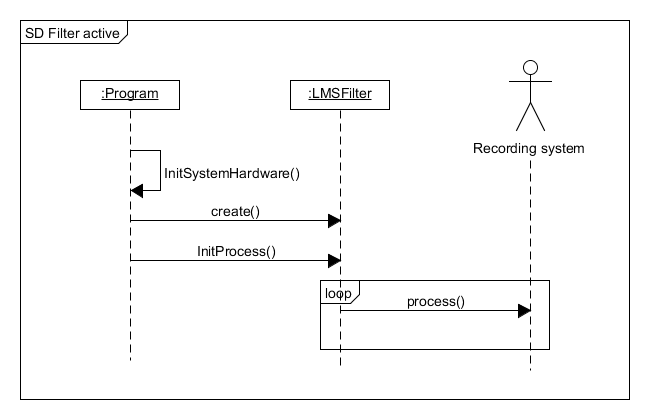
\includegraphics[width = 400pt]{Img/SD_filter_active.png}
	\caption{SD filter startes}
	\label{fig:SD}
\end{figure}
På sekvensdiagrammet ovenfor, kan man se hvordan koden køres igennem når filteret aktiveres. Process kører så længe systemet er aktivt, filtrerer uønsket støj fra og sender filtreret samples videre ud i systemet kontinuert.

%!TEX root = ../../Main.tex
\graphicspath{{Chapters/Matlab/}}
%-------------------------------------------------------------------------------







%!TEX root = ../../Main.tex
\graphicspath{{Chapters/Test/}}
%-------------------------------------------------------------------------------


\section{Test}

\subsection{Matlab simulering}

Efter den teoretiske undersøgelse, vil vi i dette afsnit udvikle og vise en simuleret version af vores filter, hvor der er taget udgangspunkt i Teori afsnittet. Da vi tager udgangspunkt i teoriafsnittet starter vi med at vise hvordan vi har implementeret vores filter. 

\begin{lstlisting}
%Create LMS FIR filter
my = 0.01; % some number 0.01
W = zeros(1,256);

for n = 1:length(d) %run every sample 
    yn = 0;
    for m = 1:length(W) %make new filteret sample 
        if n > m
            yn = yn + fixed32(W(m)*noise(n-m));
        end
    end
    y(n) = yn;
    e(n) = d(n) - y(n);
    for m = 1:length(W) %make new koefficient  
        if n > m
            W(m) = W(m) + fixed32(my*noise(n-m)*e(n));
        end
    end
end
\end{lstlisting}

Først i filteret vælger vi en my, som ift til teori afsnittet bestemmer hvor hurtig filteret er. I dette eksempel bruger vi en værdi som er testet frem til at have et god forhold mellem hastighed og settling time. Herefter bestemmes hvor mange koefficienter filteret skal have. Vi har valgt et forholdsvis højt tal, da vi simulerer. Dette vil ikke nødvendigvis være muligt på Cross-core. \\

Igennem genereringen af filteret laves der 3 forloop. Et som kører hver sample igennem, et som laver det filtrede nye sample, og et som opdaterer koefficinterne ift tilbagekoblingen. \\
De nye filter koefficienter bliver herved opdateret til det ønskede filter, hvor e(n) bliver fejlen ift figur \ref{fig:LMS_filter}, som er det talesignal der ønskes. \\
Koden er bygget op sådan at vi kører en fixed16() og fixed32(), for at simulere det bedst muligt ift blackfin. Fixed16 svarer til fixed point 1.15 og fixed32 til fixed point 1.31. 
\\
Dette giver os et filter som fungerer efter hensigten. Først testes der med 3 sinus toner, som ligger indover et tale signal, disse 3 toner skal derved gerne blive filtreret gennem filteret.

 
\newpage
\subsubsection{Første test}
Den første test der blev udført var så simpel som mulig. I forsøget generes et talesignal med 3 sinustoner indover. 
Figur \ref{fig:Filter_time} viser signalet som bliver filtreret i tidsdomænet. Her er det værd at observerer settling tiden på filteret som ses i y(n). Denne settling tid vil kunne gøres mindre ved at justere på my. Der er valgt til opgaven her at teste med 0.01 my. 
\begin{figure}[H]
	\centering
	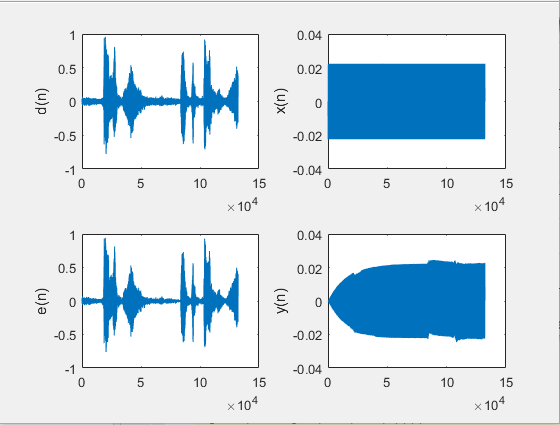
\includegraphics[width = 400pt]{Img/Filter_time}
	\caption{LMS filter i tid (3 sinus toner)}
	\label{fig:Filter_time}
\end{figure}
\newpage
Herefter vises på figur \ref{fig:Filter_Freq} signalet i frekvens domænet, her ses hvordan filteret filtrere den fejl som skabes fra, og derved skaber et signal e(n), som er talesignalet med dæmpet sinus tonerne. 

\begin{figure}[H]
	\centering
	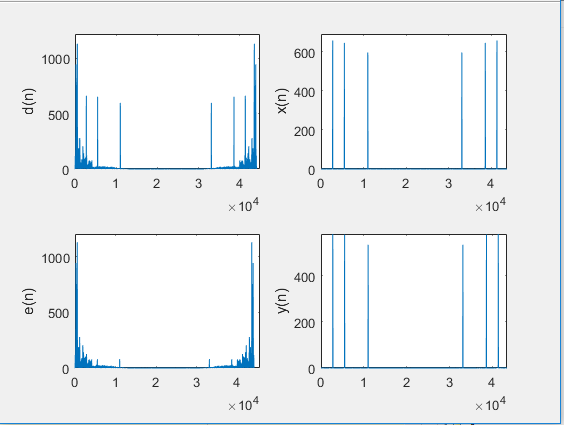
\includegraphics[width = 400pt]{Img/Filter_Freq}
	\caption{LMS filter i frekvens (3 sinus toner)}
	\label{fig:Filter_Freq}
\end{figure}
\newpage
Ved at kigge på selve filteret ses at filteret (figur \ref{fig:Filter}) skaber et filter som kun lukker de 3 sinus toner igennem, hvilket er hensigten. Dette signal bliver så fratrukket det endelige samlede signal, for at få en error som er det endelige e(n). 
\begin{figure}[H]
	\centering
	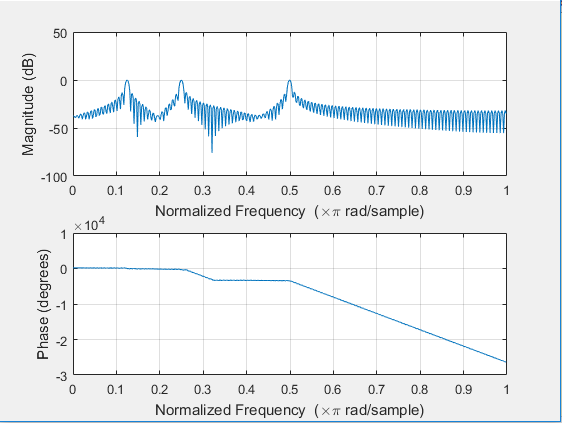
\includegraphics[width = 400pt]{Img/Filter}
	\caption{LMS filter(3 sinus toner)}
	\label{fig:Filter}
\end{figure}
\newpage
\subsubsection{Anden test}
Første test var i den nemme og simple ende, da vi kun skulle filtrere rene toner fra. Der vil i anden test forsøges at filtere en foodprocessor som bekrevet i indledningen. Denne opgave en del mere udfordrende for filteret da den nu skal filtrere mange toner og ikke kune 3, samtidig med den skal lade nogle bestemte toner gå igennem, som kommer fra talesignalet. \\
På figur \ref{fig:Filter_time_food}, ses nu det endelige produkt i tidsdomænet, der ses her en kraftig filtrering af signalet fra d(n) til e(n). Igen ser vi også en y(n) der har en settling time, inden filteret begynder at virke efter hensigten. 

\begin{figure}[H]
	\centering
	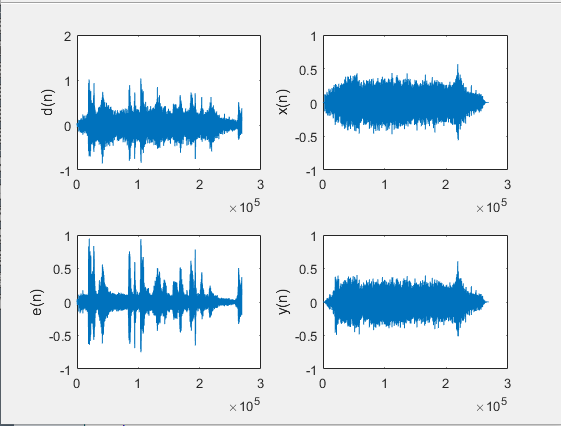
\includegraphics[width = 400pt]{Img/Filter_time_food}
	\caption{LMS filter i tid (food processor)}
	\label{fig:Filter_time_food}
\end{figure}
\newpage

Herefter tager vi et blik på frekvens donænet som viser lidt det samme billede som tidsdomænet, at LMS filteret filtrerer kraftigt fra d(n) til e(n), dette kommer af at foodprocessoren indeholder mange frekvenser. Hvis vi kigger lidt på figur \ref{fig:Filter_Freq_food}, og figur \ref{fig:Filter_food}, kan man nærstudere figur \ref{fig:Filter_food}, og se at filteret fungerer bedst når frekvenserne er udenfor talefrekvenserne, dette betyder også at filteret ikke prøver at filtrere støj fra som ligger i tale signalet, dette kan vi se fra figur \ref{fig:Filter_food}.

\begin{figure}[H]
	\centering
	\includegraphics[width = 400pt]{Img/Filter_Freq_food}
	\caption{LMS filter i frekvens (food processor)}
	\label{fig:Filter_Freq_food}
\end{figure}
\newpage

\begin{figure}[H]
	\centering
	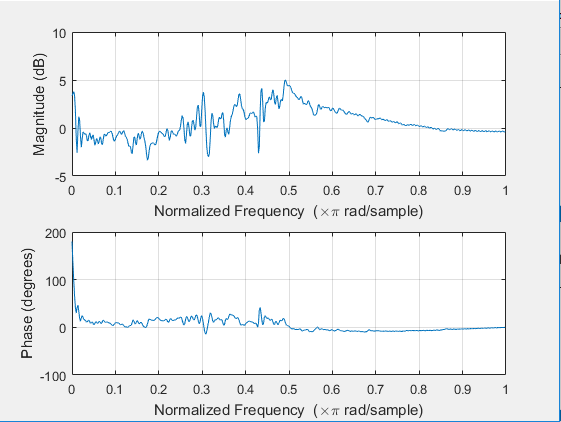
\includegraphics[width = 400pt]{Img/Filter_food}
	\caption{LMS filter(food processor)}
	\label{fig:Filter_food}
\end{figure}

\subsection{Cross-core}
\subsubsection{Overordnet}
Gruppen har valgt at lave test ud fra funktionalitet frem for use cases, da mange af use casene ikke vil godkendes, og derfor giver en forklaring af testene mere mening. 
 
\subsubsection{Visuel test}
Cross-core er et IDE, som kan programmere software over på blackfin proccesoren. Herigennem er der lavet embedded software, som styre forbindelserne på blackfin, samtidig med at vi udfører NSS's funktionalitet. Igennem undervisnignen er der blevet henvist til signal proccesering framework, som også gøres brug af i denne opgave. 

Gennem denne test var der flere ting som udfordrede funktionaliteten , og sammenligningsgrundlaget ift matlab simuleringen. 
Da det er nemmest at sammenligne med er grafer og figurer, blev vi nød til at udskrive txt filer fra blackfin, som udskrev hver sample. Da blackfin har et begrænset memory, kunne vi dog kun have 1024 sample gemt, hvilket er et meget kort lydsignal. Dette var især en ulempe, da matlab modellen var bygget op af lydsignaler med en længde på 268723 samples. Dette gør en signifikant forskel. 
Hvis vi kigger på figur \ref{fig:Blackfin}, ser vi den realiserede proces med 3 toner, som også blev brugt i matlab modellen. Dette er valgt da det visuelt er meget nemmere at se på en graf frem for støj fra en food processor.
Hvis der sammnelignes med de første 1024 samples i matlab figur \ref{fig:Blackfin_simulering}, ser vi at matlab ikke filtrerer sinus tonerne fra som ved realiseringen på blackfin. Det skal med at skaleringen af tidssignalerne fra blackfin og matlab, ikke er den samme, dette er dog blot en skaleringsfejl og værdierne er derfor stadig sammenlignelige. Det har dog ingen indflydelse på resultaterne, da skaleringen er den samme. Ydermere er der også ændret i koden, så første værdi er 1 og ikke 0, mere om det emne i diskussionen. 
\begin{figure}[H]
	\centering
	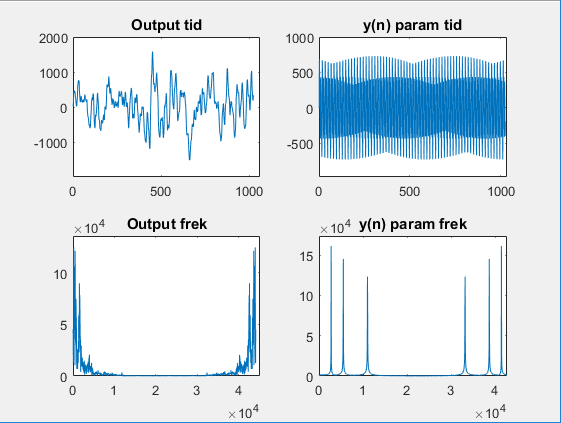
\includegraphics[width = 400pt]{Img/Blackfin}
	\caption{LMS filter implementeret på Blackfin}
	\label{fig:Blackfin}
\end{figure}

\begin{figure}[H]
	\centering
	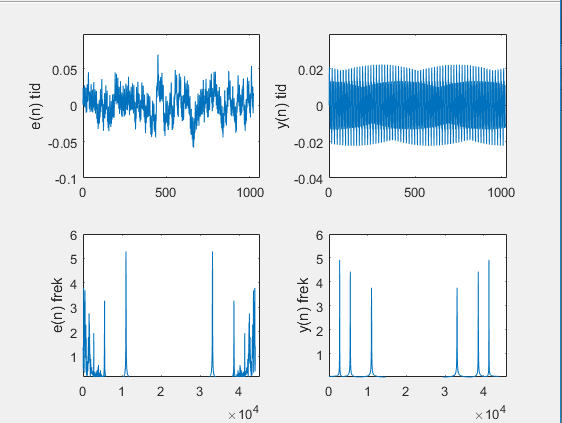
\includegraphics[width = 400pt]{Img/Blackfin_simulering}
	\caption{Simulering af figur \ref{fig:Blackfin} i matlab}
	\label{fig:Blackfin_simulering}
\end{figure}
\newpage
Hvis vi kigger nærmere på matlab simlueringen, af de samme signal og samme antal samples, undrer gruppen sig over hvordan det kan være at  matlab modellen bliver markant anderledes, og ikke ser ud til at virke efter hensigten. Dette kommer især til udtryk hvis vi kigger på figur \ref{fig:Tjek_af_frek}, hvor vi ser at frekvensen fra y(n) burde bliver trukket fra d(n), det ser dog ikke ud til at virke efter hensigten. Dette emne vil kort blive taget op i diskussionen igen. 
\begin{figure}[H]
	\centering
	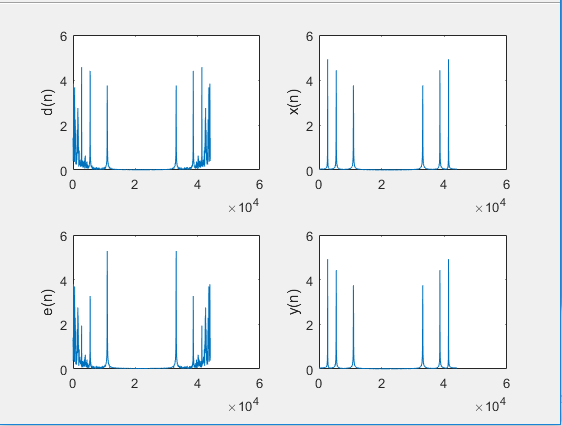
\includegraphics[width = 400pt]{Img/Tjek_af_frek}
	\caption{Fejl fra matlab filter}
	\label{fig:Tjek_af_frek}
\end{figure}

\subsubsection{Audio Test}
Gruppen har gennem testen lavet en audio test, hvor både sinus toner så vel som food processoren er blevet testet. 
Produktet og derved lyden virker til en vis grad igennem blackfin processoren. Hvis der sendes 3 sinus toner som både støj og implementeret i talesignalet, opleves at sinus tonerne fjernes, dog tilføres en "klik" lyd, som vil forsøges forklaret i diskusionen. Hvis vi derimod sender food processoren ind som støj og implementerer det i talesignal, bliver lyden forvrænget og filtrering af fejlen har ikke den ønskede funktionalitet ift at fjerne støjen. Dette vil igen blive diskuteret i diskussionen. 
%!TEX root = ../../Main.tex
\graphicspath{{Chapters/Diskussion/}}
%-------------------------------------------------------------------------------


\section{Diskussion}
Igennem processen i projektet, mødte gruppen flere problemstillinger. Noget af det første var, at bestemme hvilket filter der skulle bruges for at løse opgaven. Efter søgen på nettet og gennem undervisningsbogen, blev et LMS filter valgt som den rette løsning. Hertil er der blevet produceret et filter, som er testet både i Matlab som simulering, og på blackfin processoren som realisering. 

Igennem testen oplevede gruppen flere forskellige problemstillinger som vil redegøres for herunder. 

\begin{description}[align=left]
\item [Første sample = 1.] Igennem testen blev den første sample sat til 1 i crosscore koden, dette gøres for at få det samme signal fra input til output. Dette betyder at fejlen allerede på første sample er stor, mens hvis første sample er 0, vil filteret lige så stille og roligt få en større fejl, og derved have en indjusteringstid. Derfor giver det bedre mening at bruge en værdi på 1. Dog ser vi en at fejlen e(n) forværes hvis den første værdi i matlab koden er 1 og ikke 0. Vi har ikke nogen god forklaring på hvorfor dette er tilfældet, vi mener dog at første værdi burde være 1 for at sende det samme signal igennem. 
\item [Filter koefficienter] har stor betydning for filteret, især når vi kigger på matlab koden. For at filtrere ordentlig på de forskellige toner og food processeren, skal filteret have 256 filter koefficienter i matlab. Modsat høres væsentlig forskel på blackfin, når vi kommer over 32 koefficienter, hvor den omtalte "klik" lyd forværes, hvis vi kommer på 64 eller derover. Vi har dog ikke nogen forklaring på hvorfor matlab modellen ikke kan filtrere støjsignalerne fra ved lav filter koefficienter. Det burde være muligt at filtrere helt ned til blackfin implementeringen, især hvis man tester med 3 rene sinus toner.   
\item [Simulering af realiseringen.] 
Da der blev simuleret det eksakte som vi realiserede på blackfin, var resultaterne  ikke hvad vi forventede (figur\ref{fig:Tjek_af_frek}), da det ikke ligner at funktionen e(n) = d(n) - y(n) bliver gennemført ordentlig. Hvis man kigger på skaleringen burde filteret trække støj tonerne fra det oprindelige signal. Den bedste forklaring vi havde på dette var at der bliver brugt for lidt koefficienter, så filteret ikke lavede et filter peak på den rigtige frekvens. Dette tjekkede vi dog i matlab, og fandt at de var ens, derfor kunne den teori afvises. 
På figur \ref{fig:filter_matlab}, ser vi filteret som bliver skab i matlab, og kan derved også se at filteret ikke filtrerer de frekvenser vi regner med. Dette filter er derfor ubrugeligt. 
\begin{figure}[H]
	\centering
	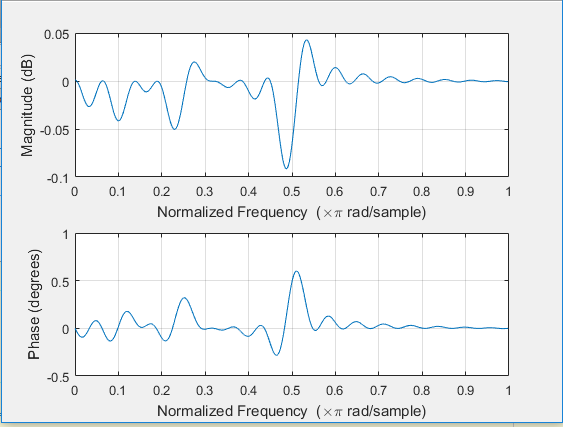
\includegraphics[width = 400pt]{Img/filter_matlab}
	\caption{Simulerings Filter af realiseringen i matlab}
	\label{fig:filter_matlab}
\end{figure}
\item [Food processor realisering] Da vi skulle teste om vores filter kunne filtrere på et mere komplekst signal end tre toner, har vi valgt at bruge en foodprocessor. Støjen fra foodprocessoren indeholder mange forskellige frekvenser, hvilket gør kravene til filteret højere. Da vi er begrænset til kun at have 32 koefficienter, begrænser det også, hvor mange frekvenser i støjsignalet, der kan dæmpes. Dette er en af grundene til at filteret ikke har haft den ønsket effekt. 
En anden grund kan også være at vores timing ikke har været god nok mellem støj signalet og tale-signalet. Da vi testede med enkelte toner fandt vi ud af at bare en lille ændring i støjsignalets frekvens gjorde filteret betydeligt dårligere til at dæmpe støjen. Så hvis timingen ikke har været præcis nok, har de forskellige frekvenser for støjsignalet ikke passet med støjen på talesignalet.
\item ["klik" lyde.] Som tidligere beskrevet opleves der "klik" lyde når filteret køres på blackfin. Den eneste gode forklaring vi har på dette, er at filterkoefficienterne ændres så hurtigt at de 'ødelægger' lyden med "klik" lyde. 
\item [Bedst udenfor 300-3400 Hz.] Vi fandt også ud af gennem projektet at LMS filteret fungerer bedst hvis det støjende signal (x(n)) og det ønskede signal (e(n)) ligger i forskellige frekvenser. Dette ses af figur \ref{fig:Filter_food}, hvor vi har et tale signal, som normalt ligger imellem 300-3400 Hz, sammensat af et food processor som støjer på et meget bredt spektrum. Det ses at filteret skaber et gain af støjen som er hensigten, når vi kommer over 3400 Hz. Dette betyder også at filteret kommer til at filtrere talesignalet, da de ligger inden for samme frekvensbånd. Dog har vi gennem projektet set at en ren sinus tone, godt kan filtreres fra selvom den ligger inderfor tale båndet. Dette skyldes højst sandsanligt at tonen er så kraftig at filteret negligere talesignalet. \\
Hvis der var uendelig processorkraft, kunne vi måske bruge krydskorralation, lave et krydskorralation på hver frekvens med støjen og derved finde peak hvor signalet og støjen korrelerer. Dette er dog ikke muligt på blackfin, da det vil bruge meget processorkraft, og memory, da hele støjsignalet ville skulle "krydses" med hele det oprindelige signal, for hver sample. 
\item [Ikke-funktionelle krav.]

I vores kravspecifikation har vi specificeret flere ikke funktionelle krav. Disse er så vidt muligt forsøgt opfyldt i vores implementering af NSS. Nogle af disse krav vil gennemgåes yderligere i dette afsnit.

System og algoritme kravene er alle opfyldt eller inden for den valgte grænse. Kravet R8(Filter algoritmen skal implementeres med fixed point), er opfyldt, da vi i vores filter gør brug af datatypen 'fract', som er en fixed point type. Kravet R9(Filteret må max bruge 10KByte memory), er ligeledes opfyldt. Dette er verificeret ved at generere et symbol map i crosscore studios. Denne fil viser hvor meget program og data memory der bliver brugt af vores filter. Ved at lægge alt data og program memory sammen for LMSFilter klassen, kan man beregne hvor mange bytes der bliver brugt. Resultatet af dette viser at der bliver brugt langt mindre end de 10KByte, der var sat som øvre grænse. Kravet R11(Filteret må max benytte 98\% DSP load), er også inden for den valgte grænse. Vi har fundet det antal cycles der bliver brugt af filteret pr. sample, hvilket giver os 3977 cycles. Dette er under grænsen på 13333 cycles, som er 98\% load. 

Tilsidst er der nogle afledte krav, der er lavet på bagrund af problemrelateret krav og system og algoritme kravene. DR3(Filter latency må max forsinkes 1280 samples(på baggrund af R6.(1/44100)*1280=30ms) er inden for grænsen. Dette skyldes antallet af filter koefficienter, som er sat til 32. Dette betyder at signalet max forsinkes 32 samples, hvilket vil sige at der er en latency på 6.6ms. 

\item [Løsning i sidste time.] Da vi stort set var færdige med rapport og kode, fandt vi en fejl i blackfin implementeringen, som forklarede og løste problemet med "klik" lydene som tidligere nævnt. 
Vi så ikke fejlen, når vi blot testede med 1024 samples, da fejlen ligger når vi tage 2,3,4.... blok af 1024 samples. Dette betyder at at vi i den tidligere kode negligerede de første 32 samples, pga funktionens if løkker. I den nye implementering, har vi derved oprettet en ny buffer som gemmer de gamle koefficienter, så de kan bruges når en ny blok af 1024 samples kommer til det første loop. Vi sikrer at vi peger det rigtige sted i bufferen, ved at sørge for, at hvis idxNew kommer under 0, sætter vi idxNew til NUM\_WEIGTHS-1, for at flippe pege pointeren op til det forrige værdi for filteret. Den nye kode kan ses herunder. Dette er et udkast til implementering, og derfor skal der også sættes tid af til at optimere koden. Vi testede herefter og fandt at "klik" lydene forsvandt. 
\newpage
\begin{lstlisting}
for(short i = 0; i < len; i++)
	{

		delay[idx] = x[i];
		idxNew = idx;
		if (++idx >= NUM_WEIGTHS) idx = 0;

		long fract yn = 0;

		for(short j = 0; j < NUM_WEIGTHS; j++)
		{
			//if(i > j)
			//{
				yn = yn + Filter.W[j]*delay[idxNew];
				if (--idxNew < 0) idxNew = NUM_WEIGTHS-1;
			//}
		}
		y[i] = (fract)yn;
		e[i] = d[i] - yn;

		long fract tmp_W = 0;

		for(short k = 0; k < NUM_WEIGTHS; k++)
		{
			if(i > k)
			{
				Filter.W[k] = Filter.W[k]  + my*x[i-k]*e[i];

			}
		}
	}
\end{lstlisting}

\item [Læringsmål.] Projektet er opbygget og leder kraftig op til læringsmålene for faget. Igennem dette projekt har vi derved undersøgt og arbejdet med hardware arkitektturen på DSP'en, dette vises og forklares gennem Struktur afsnittet. En real tids konfiguration er blevet lavet og testet gennem dette projekt, og endda til en vis grad opfyldt real tids implementeringen. Herunderover har vi udviklet og gennemarbejdet et filter som gør brug af en algoritme, herigennem LMS algoritmen, som kan ses under Teori afsnittet. Vi har ikke set meget på strømforbruget og optimering igennem dette projekt, da det ikke har været det essentielle for lige præcis dette projekt. Det vil dog kunne tages op ved efterarbejde.    


\end{description}


%!TEX root = ../../Main.tex
\graphicspath{{Chapters/Konklussion/}}
%-------------------------------------------------------------------------------


\section{Konklussion}
Igennem projektet, har vi arbejdet med simulering og realisering. Det overordnet projekt er færdiglavet med simulering, sammen med et realiseringsprojekt, som mangler finpudsning, og derved ikke er 100\% færdig implementeret. Dette betyder også at hvis produktet skulle laves færdig var det en nødvendighed, at læse denne rapport igennem og derefter gennemarbejde det sidste implementering. I sidste time af test fasen, opdagede vi en fejl, som forklarede denne "klik" lyd, som havde været et problem gennem projektets udvikling. Denne del er ret essentiel, og også vigtig i forståelsen for videre arbejde med projektet. \\
Gruppen vil derfor konkludere at projektet er gået efter hensigten ift. at udvikle, simulere, realisere og teste NSS. Den givne tidshorisont er dog blevet overskredet, og derfor ligger der endnu nogle timer for at få projektet gennemført. Derudover mener vi at der er opfyldt læringsmål, så vel som veldokumenteret rapport til at dokumentere vores resultat afsnit, som opfordrer til diskussion. 


\begin{flushleft}
	
\end{flushleft}


\bibliographystyle{plain}
\bibliography{Bibliography}	

\begin{thebibliography}{9}

\bibitem{Teori} 
Gan and Kuo. \\
\textit{Embedded Signal Processing with the Micro Signal Architecture, Chapter 4.4.1}\\ 
John Wiley 1st Ed. 2007.
 
\bibitem{Struktur} 
Gan and Kuo. \\
\textit{Embedded Signal Processing with the Micro Signal Architecture, Chapter 7.2.2.1}\\ 
John Wiley 1st Ed. 2007.
  
\end{thebibliography}

\end{document}